% !TeX spellcheck = en_US
\documentclass[10pt,journal,compsoc]{IEEEtran}
%
% If IEEEtran.cls has not been installed into the LaTeX system files,
% manually specify the path to it like:
% \documentclass[10pt,journal,compsoc]{../sty/IEEEtran}





% Some very useful LaTeX packages include:
% (uncomment the ones you want to load)


% *** MISC UTILITY PACKAGES ***
%
%\usepackage{ifpdf}
% Heiko Oberdiek's ifpdf.sty is very useful if you need conditional
% compilation based on whether the output is pdf or dvi.
% usage:
% \ifpdf
%   % pdf code
% \else
%   % dvi code
% \fi
% The latest version of ifpdf.sty can be obtained from:
% http://www.ctan.org/pkg/ifpdf
% Also, note that IEEEtran.cls V1.7 and later provides a builtin
% \ifCLASSINFOpdf conditional that works the same way.
% When switching from latex to pdflatex and vice-versa, the compiler may
% have to be run twice to clear warning/error messages.






% *** CITATION PACKAGES ***
%
\ifCLASSOPTIONcompsoc
  % IEEE Computer Society needs nocompress option
  % requires cite.sty v4.0 or later (November 2003)
  \usepackage[nocompress]{cite}
\else
  % normal IEEE
  \usepackage{cite}
\fi
% cite.sty was written by Donald Arseneau
% V1.6 and later of IEEEtran pre-defines the format of the cite.sty package
% \cite{} output to follow that of the IEEE. Loading the cite package will
% result in citation numbers being automatically sorted and properly
% "compressed/ranged". e.g., [1], [9], [2], [7], [5], [6] without using
% cite.sty will become [1], [2], [5]--[7], [9] using cite.sty. cite.sty's
% \cite will automatically add leading space, if needed. Use cite.sty's
% noadjust option (cite.sty V3.8 and later) if you want to turn this off
% such as if a citation ever needs to be enclosed in parenthesis.
% cite.sty is already installed on most LaTeX systems. Be sure and use
% version 5.0 (2009-03-20) and later if using hyperref.sty.
% The latest version can be obtained at:
% http://www.ctan.org/pkg/cite
% The documentation is contained in the cite.sty file itself.
%
% Note that some packages require special options to format as the Computer
% Society requires. In particular, Computer Society  papers do not use
% compressed citation ranges as is done in typical IEEE papers
% (e.g., [1]-[4]). Instead, they list every citation separately in order
% (e.g., [1], [2], [3], [4]). To get the latter we need to load the cite
% package with the nocompress option which is supported by cite.sty v4.0
% and later. Note also the use of a CLASSOPTION conditional provided by
% IEEEtran.cls V1.7 and later.





% *** GRAPHICS RELATED PACKAGES ***
%
\ifCLASSINFOpdf
  \usepackage[pdftex,final]{graphicx}
  % declare the path(s) where your graphic files are
  \graphicspath{{../pdf/}{../jpeg/}}
  % and their extensions so you won't have to specify these with
  % every instance of \includegraphics
  \DeclareGraphicsExtensions{.pdf,.jpeg,.png}
\else
  % or other class option (dvipsone, dvipdf, if not using dvips). graphicx
  % will default to the driver specified in the system graphics.cfg if no
  % driver is specified.
  \usepackage[dvips]{graphicx}
  % declare the path(s) where your graphic files are
  \graphicspath{{../eps/}}
  % and their extensions so you won't have to specify these with
  % every instance of \includegraphics
  \DeclareGraphicsExtensions{.eps}
\fi
% graphicx was written by David Carlisle and Sebastian Rahtz. It is
% required if you want graphics, photos, etc. graphicx.sty is already
% installed on most LaTeX systems. The latest version and documentation
% can be obtained at: 
% http://www.ctan.org/pkg/graphicx
% Another good source of documentation is "Using Imported Graphics in
% LaTeX2e" by Keith Reckdahl which can be found at:
% http://www.ctan.org/pkg/epslatex
%
% latex, and pdflatex in dvi mode, support graphics in encapsulated
% postscript (.eps) format. pdflatex in pdf mode supports graphics
% in .pdf, .jpeg, .png and .mps (metapost) formats. Users should ensure
% that all non-photo figures use a vector format (.eps, .pdf, .mps) and
% not a bitmapped formats (.jpeg, .png). The IEEE frowns on bitmapped formats
% which can result in "jaggedy"/blurry rendering of lines and letters as
% well as large increases in file sizes.
%
% You can find documentation about the pdfTeX application at:
% http://www.tug.org/applications/pdftex






% *** MATH PACKAGES ***
%
\usepackage{amsmath}
% A popular package from the American Mathematical Society that provides
% many useful and powerful commands for dealing with mathematics.
%
% Note that the amsmath package sets \interdisplaylinepenalty to 10000
% thus preventing page breaks from occurring within multiline equations. Use:
%\interdisplaylinepenalty=2500
% after loading amsmath to restore such page breaks as IEEEtran.cls normally
% does. amsmath.sty is already installed on most LaTeX systems. The latest
% version and documentation can be obtained at:
% http://www.ctan.org/pkg/amsmath





% *** SPECIALIZED LIST PACKAGES ***
%
%\usepackage{algorithmic}
% algorithmic.sty was written by Peter Williams and Rogerio Brito.
% This package provides an algorithmic environment fo describing algorithms.
% You can use the algorithmic environment in-text or within a figure
% environment to provide for a floating algorithm. Do NOT use the algorithm
% floating environment provided by algorithm.sty (by the same authors) or
% algorithm2e.sty (by Christophe Fiorio) as the IEEE does not use dedicated
% algorithm float types and packages that provide these will not provide
% correct IEEE style captions. The latest version and documentation of
% algorithmic.sty can be obtained at:
% http://www.ctan.org/pkg/algorithms
% Also of interest may be the (relatively newer and more customizable)
% algorithmicx.sty package by Szasz Janos:
% http://www.ctan.org/pkg/algorithmicx




% *** ALIGNMENT PACKAGES ***
%
\usepackage{array}
% Frank Mittelbach's and David Carlisle's array.sty patches and improves
% the standard LaTeX2e array and tabular environments to provide better
% appearance and additional user controls. As the default LaTeX2e table
% generation code is lacking to the point of almost being broken with
% respect to the quality of the end results, all users are strongly
% advised to use an enhanced (at the very least that provided by array.sty)
% set of table tools. array.sty is already installed on most systems. The
% latest version and documentation can be obtained at:
% http://www.ctan.org/pkg/array


% IEEEtran contains the IEEEeqnarray family of commands that can be used to
% generate multiline equations as well as matrices, tables, etc., of high
% quality.




% *** SUBFIGURE PACKAGES ***
%\ifCLASSOPTIONcompsoc
%  \usepackage[caption=false,font=footnotesize,labelfont=sf,textfont=sf]{subfig}
%\else
%  \usepackage[caption=false,font=footnotesize]{subfig}
%\fi
% subfig.sty, written by Steven Douglas Cochran, is the modern replacement
% for subfigure.sty, the latter of which is no longer maintained and is
% incompatible with some LaTeX packages including fixltx2e. However,
% subfig.sty requires and automatically loads Axel Sommerfeldt's caption.sty
% which will override IEEEtran.cls' handling of captions and this will result
% in non-IEEE style figure/table captions. To prevent this problem, be sure
% and invoke subfig.sty's "caption=false" package option (available since
% subfig.sty version 1.3, 2005/06/28) as this is will preserve IEEEtran.cls
% handling of captions.
% Note that the Computer Society format requires a sans serif font rather
% than the serif font used in traditional IEEE formatting and thus the need
% to invoke different subfig.sty package options depending on whether
% compsoc mode has been enabled.
%
% The latest version and documentation of subfig.sty can be obtained at:
% http://www.ctan.org/pkg/subfig




% *** FLOAT PACKAGES ***
%
%\usepackage{fixltx2e}
% fixltx2e, the successor to the earlier fix2col.sty, was written by
% Frank Mittelbach and David Carlisle. This package corrects a few problems
% in the LaTeX2e kernel, the most notable of which is that in current
% LaTeX2e releases, the ordering of single and double column floats is not
% guaranteed to be preserved. Thus, an unpatched LaTeX2e can allow a
% single column figure to be placed prior to an earlier double column
% figure.
% Be aware that LaTeX2e kernels dated 2015 and later have fixltx2e.sty's
% corrections already built into the system in which case a warning will
% be issued if an attempt is made to load fixltx2e.sty as it is no longer
% needed.
% The latest version and documentation can be found at:
% http://www.ctan.org/pkg/fixltx2e


%\usepackage{stfloats}
% stfloats.sty was written by Sigitas Tolusis. This package gives LaTeX2e
% the ability to do double column floats at the bottom of the page as well
% as the top. (e.g., "\begin{figure}[!b]" is not normally possible in
% LaTeX2e). It also provides a command:
%\fnbelowfloat
% to enable the placement of footnotes below bottom floats (the standard
% LaTeX2e kernel puts them above bottom floats). This is an invasive package
% which rewrites many portions of the LaTeX2e float routines. It may not work
% with other packages that modify the LaTeX2e float routines. The latest
% version and documentation can be obtained at:
% http://www.ctan.org/pkg/stfloats
% Do not use the stfloats baselinefloat ability as the IEEE does not allow
% \baselineskip to stretch. Authors submitting work to the IEEE should note
% that the IEEE rarely uses double column equations and that authors should try
% to avoid such use. Do not be tempted to use the cuted.sty or midfloat.sty
% packages (also by Sigitas Tolusis) as the IEEE does not format its papers in
% such ways.
% Do not attempt to use stfloats with fixltx2e as they are incompatible.
% Instead, use Morten Hogholm'a dblfloatfix which combines the features
% of both fixltx2e and stfloats:
%
% \usepackage{dblfloatfix}
% The latest version can be found at:
% http://www.ctan.org/pkg/dblfloatfix




\ifCLASSOPTIONcaptionsoff
  \usepackage[nomarkers]{endfloat}
 \let\MYoriglatexcaption\caption
 \renewcommand{\caption}[2][\relax]{\MYoriglatexcaption[#2]{#2}}
\fi
% endfloat.sty was written by James Darrell McCauley, Jeff Goldberg and 
% Axel Sommerfeldt. This package may be useful when used in conjunction with 
% IEEEtran.cls'  captionsoff option. Some IEEE journals/societies require that
% submissions have lists of figures/tables at the end of the paper and that
% figures/tables without any captions are placed on a page by themselves at
% the end of the document. If needed, the draftcls IEEEtran class option or
% \CLASSINPUTbaselinestretch interface can be used to increase the line
% spacing as well. Be sure and use the nomarkers option of endfloat to
% prevent endfloat from "marking" where the figures would have been placed
% in the text. The two hack lines of code above are a slight modification of
% that suggested by in the endfloat docs (section 8.4.1) to ensure that
% the full captions always appear in the list of figures/tables - even if
% the user used the short optional argument of \caption[]{}.
% IEEE papers do not typically make use of \caption[]'s optional argument,
% so this should not be an issue. A similar trick can be used to disable
% captions of packages such as subfig.sty that lack options to turn off
% the subcaptions:
% For subfig.sty:
% \let\MYorigsubfloat\subfloat
% \renewcommand{\subfloat}[2][\relax]{\MYorigsubfloat[]{#2}}
% However, the above trick will not work if both optional arguments of
% the \subfloat command are used. Furthermore, there needs to be a
% description of each subfigure *somewhere* and endfloat does not add
% subfigure captions to its list of figures. Thus, the best approach is to
% avoid the use of subfigure captions (many IEEE journals avoid them anyway)
% and instead reference/explain all the subfigures within the main caption.
% The latest version of endfloat.sty and its documentation can obtained at:
% http://www.ctan.org/pkg/endfloat
%
% The IEEEtran \ifCLASSOPTIONcaptionsoff conditional can also be used
% later in the document, say, to conditionally put the References on a 
% page by themselves.




% *** PDF, URL AND HYPERLINK PACKAGES ***
%
\usepackage{url}
% url.sty was written by Donald Arseneau. It provides better support for
% handling and breaking URLs. url.sty is already installed on most LaTeX
% systems. The latest version and documentation can be obtained at:
% http://www.ctan.org/pkg/url
% Basically, \url{my_url_here}.





% *** Do not adjust lengths that control margins, column widths, etc. ***
% *** Do not use packages that alter fonts (such as pslatex).         ***
% There should be no need to do such things with IEEEtran.cls V1.6 and later.
% (Unless specifically asked to do so by the journal or conference you plan
% to submit to, of course. )


% correct bad hyphenation here
\hyphenation{op-tical net-works Wiki-Leaks}

%%%%%%%%%%%%%%%%%%%%%%%%%%%%%%%%%%%%%%%%%%%%%%%%%%%%%%%%%%%%
%% Custom Packages not from the template
%%%%%%%%%%%%%%%%%%%%%%%%%%%%%%%%%%%%%%%%%%%%%%%%%%%%%%%%%%%%
\usepackage{nth}
\usepackage[hidelinks]{hyperref}

% Document annotations
\usepackage[nomargin,draft]{fixme}
\fxsetup{layout=pdfnote}

\usepackage{fixfoot}


\begin{document}
%
% paper title
% Titles are generally capitalized except for words such as a, an, and, as,
% at, but, by, for, in, nor, of, on, or, the, to and up, which are usually
% not capitalized unless they are the first or last word of the title.
% Linebreaks \\ can be used within to get better formatting as desired.
% Do not put math or special symbols in the title.
\title{Unobservable Messaging with MessageVortex}
%
%
% author names and IEEE memberships
% note positions of commas and nonbreaking spaces ( ~ ) LaTeX will not break
% a structure at a ~ so this keeps an author's name from being broken across
% two lines.
% use \thanks{} to gain access to the first footnote area
% a separate \thanks must be used for each paragraph as LaTeX2e's \thanks
% was not built to handle multiple paragraphs
%
%
%\IEEEcompsocitemizethanks is a special \thanks that produces the bulleted
% lists the Computer Society journals use for "first footnote" author
% affiliations. Use \IEEEcompsocthanksitem which works much like \item
% for each affiliation group. When not in compsoc mode,
% \IEEEcompsocitemizethanks becomes like \thanks and
% \IEEEcompsocthanksitem becomes a line break with idention. This
% facilitates dual compilation, although admittedly the differences in the
% desired content of \author between the different types of papers makes a
% one-size-fits-all approach a daunting prospect. For instance, compsoc 
% journal papers have the author affiliations above the "Manuscript
% received ..."  text while in non-compsoc journals this is reversed. Sigh.

\author{Martin~Gwerder%,~\IEEEmembership{Member,~IEEE,}
        %John~Doe,~\IEEEmembership{Fellow,~OSA,}

\IEEEcompsocitemizethanks{\IEEEcompsocthanksitem M. Gwerder was with the Institute of Mobile and Distributed Systems
of the University of Applied Sciences of Northwestern Switzerland.\protect\\
% note need leading \protect in front of \\ to get a newline within \thanks as
% \\ is fragile and will error, could use \hfil\break instead.
E-mail: see http://www.messagevortex.net
%\IEEEcompsocthanksitem J. Doe and J. Doe are with Anonymous University.
}% <-this % stops an unwanted space
\thanks{Manuscript received June 1, 2019; revised July 20, 2019.}
        }% <-this % stops a space

% note the % following the last \IEEEmembership and also \thanks - 
% these prevent an unwanted space from occurring between the last author name
% and the end of the author line. i.e., if you had this:
% 
% \author{....lastname \thanks{...} \thanks{...} }
%                     ^------------^------------^----Do not want these spaces!
%
% a space would be appended to the last name and could cause every name on that
% line to be shifted left slightly. This is one of those "LaTeX things". For
% instance, "\textbf{A} \textbf{B}" will typeset as "A B" not "AB". To get
% "AB" then you have to do: "\textbf{A}\textbf{B}"
% \thanks is no different in this regard, so shield the last } of each \thanks
% that ends a line with a % and do not let a space in before the next \thanks.
% Spaces after \IEEEmembership other than the last one are OK (and needed) as
% you are supposed to have spaces between the names. For what it is worth,
% this is a minor point as most people would not even notice if the said evil
% space somehow managed to creep in.



% The paper headers
\markboth{IEEE Transactions on Information Forensics and Security,~Vol.~XXXX, No.~XXXX, September~2019}%
{Gwerder \MakeLowercase{\textit{et al.}}: Unobservable Messaging wit Messagevortex}
% The only time the second header will appear is for the odd numbered pages
% after the title page when using the twoside option.
% 
% *** Note that you probably will NOT want to include the author's ***
% *** name in the headers of peer review papers.                   ***
% You can use \ifCLASSOPTIONpeerreview for conditional compilation here if
% you desire.



% The publisher's ID mark at the bottom of the page is less important with
% Computer Society journal papers as those publications place the marks
% outside of the main text columns and, therefore, unlike regular IEEE
% journals, the available text space is not reduced by their presence.
% If you want to put a publisher's ID mark on the page you can do it like
% this:
%\IEEEpubid{0000--0000/00\$00.00~\copyright~2015 IEEE}
% or like this to get the Computer Society new two part style.
%\IEEEpubid{\makebox[\columnwidth]{\hfill 0000--0000/00/\$00.00~\copyright~2015 IEEE}%
%\hspace{\columnsep}\makebox[\columnwidth]{Published by the IEEE Computer Society\hfill}}
% Remember, if you use this you must call \IEEEpubidadjcol in the second
% column for its text to clear the IEEEpubid mark (Computer Society jorunal
% papers don't need this extra clearance.)



% use for special paper notices
%\IEEEspecialpapernotice{(Invited Paper)}



% for Computer Society papers, we must declare the abstract and index terms
% PRIOR to the title within the \IEEEtitleabstractindextext IEEEtran
% command as these need to go into the title area created by \maketitle.
% As a general rule, do not put math, special symbols or citations
% in the abstract or keywords.
\IEEEtitleabstractindextext{%
\begin{abstract}
In this paper, we introduce an unobservable message anonymization protocol, named MessageVortex. It bases on the zero trust principle and a distributed peer-to-peer like architecture and avoids central aspects such as fixed infrastructures within a global network. 

It scores over existing work by blending its traffic into suitable existing transport protocols, thus making it next to impossible to block it without significantly affecting regular users of the transport medium. No additional protocol-specific infrastructure is required in public networks and allows a sender to control all aspects of a message such as the degree of anonymity, timing, and redundancy of the message transport without disclosing any of these details to the routing or transporting nodes. The most recent RFC-draft describes the protocol in detail. This draft contains all the necessary information to build protocol nodes. 
\end{abstract}

% Note that keywords are not normally used for peerreview papers.
\begin{IEEEkeywords}
Anonymity, Unlinkability, Communication protocol, Steganography
\end{IEEEkeywords}}


% make the title area
\maketitle


% To allow for easy dual compilation without having to reenter the
% abstract/keywords data, the \IEEEtitleabstractindextext text will
% not be used in maketitle, but will appear (i.e., to be "transported")
% here as \IEEEdisplaynontitleabstractindextext when the compsoc 
% or transmag modes are not selected <OR> if conference mode is selected 
% - because all conference papers position the abstract like regular
% papers do.
\IEEEdisplaynontitleabstractindextext
% \IEEEdisplaynontitleabstractindextext has no effect when using
% compsoc or transmag under a non-conference mode.



% For peer review papers, you can put extra information on the cover
% page as needed:
% \ifCLASSOPTIONpeerreview
% \begin{center} \bfseries EDICS Category: 3-BBND \end{center}
% \fi
%
% For peerreview papers, this IEEEtran command inserts a page break and
% creates the second title. It will be ignored for other modes.
\IEEEpeerreviewmaketitle



\IEEEraisesectionheading{\section{Introduction}\label{sec:introduction}}
% Computer Society journal (but not conference!) papers do something unusual
% with the very first section heading (almost always called "Introduction").
% They place it ABOVE the main text! IEEEtran.cls does not automatically do
% this for you, but you can achieve this effect with the provided
% \IEEEraisesectionheading{} command. Note the need to keep any \label that
% is to refer to the section immediately after \section in the above as
% \IEEEraisesectionheading puts \section within a raised box.




% The very first letter is a 2 line initial drop letter followed
% by the rest of the first word in caps (small caps for compsoc).
% 
% form to use if the first word consists of a single letter:
% \IEEEPARstart{A}{demo} file is ....
% 
% form to use if you need the single drop letter followed by
% normal text (unknown if ever used by the IEEE):
% \IEEEPARstart{A}{}demo file is ....
% 
% Some journals put the first two words in caps:
% \IEEEPARstart{T}{his demo} file is ....
% 
% Here we have the typical use of a "T" for an initial drop letter
% and "HIS" in caps to complete the first word.
\IEEEPARstart{A}{lmon Brown Strowger} was the owner of a funeral parlor in St. Petersburg. He filed a patent on March \nth{10}, 1891 for an ``Automatic Telephone Exchange'' \cite{pulseDialingPatent}. This patent built the base for modern automated telephone systems. According to several sources, he was annoyed by the fact that the local telephone operator was married to another undertaker. She diverted potential customers of Mr. Strowger to her husband instead, which caused Almon B. Strowger to lose business. In 1922, this telephone dialing system, which is nowadays called pulse dialing became the standard dialing technology for more than 70 years until tone dialing replaced it.

This dialing technology enabled automatic routing for voice and text messages (e.g., telex) up until today and is one of the foundations for our current routed networks. These networks build the base of our communication-based Society these days and allow us to connect quickly with any person or company of our wish. We use these networks today as communication meaning for all purposes, and most of the people spend minimal thoughts on the possible consequences arising if someone puts hands on this communication. 

Collected data may be used to judge upon our intentions and thus is not only confidential if we have something to hide. This problem has dramatically increased in the last years as big companies and countries started to collect all kinds of data and created the means to process them. Such a judgment allows, supposedly, to classify people and their intentions. This is not limited to what they are doing but as well, on what they did and what they might do. Numerous events in the present and past show that multiple actors, some of which are state-sponsored, collected data on a broad base within the Internet. Whether this is a problem or not may be disputable. Undisputed is that such data requires careful handling, and accusations should then base on solid facts. Unacceptable seems the use of ``guesses'' or ``extrapolations'' in most of the cases.

To show that this may happen even under complete democratic control, we may refer to events such as the ``secret files scandal'' (or  ``Fichenskandal'') in Switzerland. In the years from 1900 to 1990 Swiss government collected 900’000 files in a secret archive (covering roughly 10\% of the natural and juristic entities within Switzerland at that time)\cite{Leuenberger1989}.

Whistleblower Edward Snowden leaked a vast amount of documents. These documents suggested that such attacks on privacy are commonly made on a global scale. The documents leaked in 2009 and a significant number of journalists from multiple countries screened them (e.g., \cite{NCR2013}, \cite{XKeyscore}, \cite{Ball2013} or \cite{Greenberg2013}). According to these documents, NSA infiltrated more than 50k computer networks with malware to collect classified or personal information. They furthermore infiltrated Telecom-Operators (according to the same documents mainly executed by British GCHQ) such as Belgacom to collect data and targeted high member of governments even in associated states (such as the mobile phone number of Germany's president and high ranking members of economy and finance).

The National Security Agency (NSA) collected network data with a program called XKeyscore. Several proofs and in-depth information have been found within the documents leaked by Snowden (e.g., \cite{XKeyscore}). According to these papers, XKeyscore spanned (in 2008) $\approx150$ sites with $700$ Severs collecting emails, web traffic, and chat messages.

This list of events shows that big players are collecting and storing vast amounts of data for immediate or possible future analysis. The list of events also shows that the use of this data has in the past been at least partially questionable. As a part of possible countermeasures, this work analyses the possibility of using state-of-the-art technology to minimize the information footprint of a person on the Internet. 

We leave a large information footprint in our daily communication. On a regular email, we disclose everything in a ``postcard'' to any entity on its way. Even when encrypting a message perfectly with today's technology (S/MIME\cite{RFC2045} or PGP\cite{RFC2015}) it still leaves at least the originating and the receiving entity disclosed, or we rely on the promises of a third party provider which offers a proprietary solution. Even in those cases, we leak pieces of information such as ``message subject'', ``frequency of exchanged messages'', ``size of messages'', or ``client being used''. This meta information may leak properties such as the intensity of relationships or group memberships. A suitable anonymity protocol has, therefore, not only a message to hide but additional attributes as well. It includes leaving the message itself aside, all metadata, and all the traffic flows. Furthermore, a protocol to unlink and anonymize messages should not rely on the trust of infrastructure other than the infrastructure under control of the sending or receiving entity. Trust in any third party might be misleading in terms of security of the protocol.

Central infrastructure is bound to be of particular interest to anyone gathering data. It may furthermore allow manipulating the system or the data or the data flow. So, avoiding a central infrastructure was a primary goal for our protocol.

Leaving no information trail when sending information from one person to another is hard to achieve. Most messaging systems disclose at least the peer partners when sending messages. Metadata such as starting and endpoints, frequency, or message size are leaked in messaging systems such as XMPP, IRC, email, or Whatsapp even when encrypting messages.

Allowing an entity to collect data may affect senders and recipients of any information. Collection of vast amounts of data allows a potent adversary to build a  profile of a person. Unlike in the past, the availability of this kind of information has been risen to a never known extend with the Internet.

An entity in possession of such Profiles may use them for many purposes. These include service adoption, directed advertising, or classification of citizens. The examples given above show that the effects of this data is not limited to the Internet but reaches us effectively in the real world. While directed advertising may be classified as legit use, a general classification of citizens was considered as unacceptable in the past (see previously quoted documents \cite{NCR2013}, \cite{XKeyscore}, \cite{Ball2013}, \cite{Greenberg2013},\cite{Leuenberger1989})

The main problem of this data is that it may be collected over a considerable amount of time and evaluated at any time. It even happened that standard practices of the time are judged differently upon later. Persons may then be judged retrospectively upon these types of practice. This questionable type of judgment is visible in the tax avoidance discussion\cite{Amat1999}. 

People must be able to control their data footprint. Not providing these means does effectively allow any country or a bigger player to ban and control any number of persons within or outside the Internet.  

In this work, a new protocol is designed to allow message transfer through existing communication channels. These messages are next to unobservable for any third party. This unobservability does not only cover the message itself but all metadata and flows associated with it. We called this protocol ``MessageVortex'' or in short just ``Vortex''. The protocol is designed in such a way so that it is capable of using a wide variety of transport protocols. It is even possible to switch protocols while the messages are transferred. This behavior allows media breaches (at least on a protocol level) and makes analysis even harder.

The new protocol allows secure communication without the need for trusting the underlying transport media. Furthermore, the usage of the protocol itself is possible without altering the immediate behavior of the transport layer. That way it is possible to use the transport layers regular traffic to increase the noise in which information has to be searched. 

\subsection{About Unlinkability, Unobservability, Undetectability and Censorship resistance}
For definition of terms ``unlinkability'', ``anonymity'', and ``undetectability'', we use definitions as provided by \cite{anon_terminology}. From an academic point of view, achieving anonymity is relatively simple. All we need is a trusted party distributing the messages while making sure that no trace from the sender arrives at the recipient. Unlinkability is much harder to achieve. It requires that a specified attacker is unable to link a sender and recipients of a message. A soon as a system provides properties identifiable by third parties, it is prone to denial of service and thus partial or full censorship. By introducing a global observer or infiltrating parts of the system, an attacker may gain insight into the messages transported by the system and thus leaking information.

So to be censorship resistant, a protocol requires many critical, unobvious properties. As outlined, it should be undetectable from the outside. From within the system, we need to provide a mean to make it very hard, or ideally impossible to follow message flows or identify participants.

MessageVortex is a protocol providing censorship resistance under ideal circumstances. It does this using a rigid design from bottom up to provide the required properties. While being a protocol on its own, it uses many standard protocols. Partly to provide user-friendliness, but mostly to hide within the regular network flows. As such, a protocol requires to be undetectable on the network. A protocol all alone may not be undetectable as each protocol sends data over a network. This data is detectable. A protocol sending undetectable data, a censorship-resistant protocol requires to be embedded undetectably in legit message flows or hide in side channels. Such embedding is usually done either by side channel transmissions or by employing steganography. Our protocol may use both. The steganography is, however, the preferred way as it implies no control over the transport infrastructure.

\subsection{Adversary Model}
We refer to jurisdiction as a geographical area where a set of legal rules created by a single actor or a group of actors apply and contains executive means to enforce this set of legal rules.

We assume that the most potent adversaries are state-sponsored actors. Such actors may have high funding and are assumed to have elaborated capabilities within the jurisdiction of the sponsor. State-sponsored actors may work with allies. Achieving dominance on a world scale is excluded from our model. We always assume one or more actors with disjoint interests covering half of the network or more. We, furthermore, assume that there are always neutral actors not having  disjoint interests

We assume the following goals for an adversary:
\begin{itemize}
	\item An adversary may want to disrupt non-authorized communication.
	\item An adversary may want to read any information passing throughout the Internet.
	\item An adversary may want to build and conserve data about individuals or groups of individuals of their life. This data includes all activities in any part of their life regardless of their apparent fitness for any specific purpose or their correctness.
\end{itemize}

To achieve these goals, we assume the following properties of our adversary:
\begin{itemize}
	\item An adversary has elaborated technical know-how to attack any infrastructure. This attack may cover any attack favoring his goals, starting with exploiting weaknesses of popular software (e.g., buffer overflows or zero-day exploits) down to simple or elaborated (D)DoS attacks.
	\item An adversary may have the capability to monitor traffic at any point in public networks within a jurisdiction.
	\item An adversary may have the capability to modify routing information within a jurisdiction freely.
	\item An adversary may have the possibility to freely modify even cryptographically weak secured data where a single or a limited number of entities grant proof of authenticity or privacy.
	\item An adversary may have the possibility to inject or modify any data on the network of a jurisdiction.
	\item An adversary may create own nodes of a network. He may furthermore monitor their behavior and data flow without limitation.
	\item An adversary may force a limited number of other non-allied nodes to expose their data to him. Actors with disjoint interests are explicitly excluded from this assumption.
	\item An adversary may have similar access to resources as within its jurisdiction in a limited number of other jurisdictions.
\end{itemize}

We may test this adversary by taking a known, strong adversary. This adversary is much more potent than the supposed XKeyscore application. It surpasses the XKeyscore in terms of observation capabilities and routing. The Snowden papers suggest that this type of adversary is generally realistic, but even the supposedly most powerful country in the world was unable to set up such an adversary.

\subsection{Notation \label{sec:encNot}}
The theory in this document is heavily based on symmetric encryption, asymmetric encryption, and cryptographic hashing. To use a uniformed notation, we use $E^{K_a}(M)$ (where $a$ is an index to distinguish multiple keys) for an encrypting function with a key $K_a$. This results in $\mathbf{M^{K_a}}$ for the encrypted message. If we are reflecting a tuple of information, we write in boldface. To express a concatenated set of information, we use angular brackets $\mathbf{\langle normalAddress,vortexAddress\rangle }$. 

For a symmetric encryption of a message $\mathbf{M}$ with a key $K_a$ resulting in $\mathbf{M^{K_a}}$ where $a$ is an index to distinguish different keys. Decryption uses therefore $D^{K_a}(\mathbf{M^{K_a}})=\mathbf{M}$.

As notation for asymmetric encryption we use $E^{K^{1}_a}(\mathbf{M})$ where as $K^{-1}_a$ is the private key and $K^{1}_a$ is the public key of a key pair $K^p_a$. The asymmetric decryption is noted as $D^{K^{-1}_a}(\mathbf{M})$.

For hashing, we do use $H(\mathbf{M})$ if unsalted and $H^{S_a}$ if using a salted hash with salt $S_a$. The generated hash is shown as $H_M$ if unsalted and $H^{S_a}_M$ if salted.

If we want to express what details contained in a tuple we use the the notation $\mathbf{M\langle t,MURB,serial\rangle }$ respectively if encrypted $\mathbf{M^{K_{a}}\langle t,MURB,serial\rangle}$.

\begin{align*}
\text{asymmetric:}         & E^{K^{-1}_a}\left(\mathbf{M}\right)                            && =\mathbf{M}^{K^{-1}_a}\\
& D^{K^{1}_a}\left(E^{K^{-1}_a}\left(\mathbf{M}\right)\right)    && =\mathbf{M}\\
& D^{K^{-1}_a}\left(E^{K^{1}_a}\left(\mathbf{M}\right)\right)    && =\mathbf{M}\\
\text{symmetric:}          & E^{K_a}\left(\mathbf{M}\right)                                 && =\mathbf{M}^{K_a}\\
& D^{K_a}\left(E^{K_a}\left(\mathbf{M}\right)\right)          && =\mathbf{M}\\
\text{hashing (unsalted):}& H\left(\mathbf{M}\right)                                       && =\mathbf{H}_M\\
\text{hashing (salted):}  & H^{S_a}\left(\mathbf{M}\right)                                 && =\mathbf{H}^{S_a}_M
\end{align*}

In general, subscripts denote selectors to differentiate values of the same type, and superscript denotes relevant parameters to operations expressed. The subscripted and superscripted information may be omitted where not needed.

We refer to the encrypted components of a Vortex Message as follows:
\begin{align*}
\text{Prefix component:}         & \mathbf{PREFIX}                 &=D^{K^{1}_a}\left(\mathbf{P}^{K^{-1}_a}\right) &=D\left(\mathbf{P}\right)\\
\text{Header component:}         & \mathbf{HEAD}                 &=D^{K^{1}_a}\left(\mathbf{H}^{K^{-1}_a}\right) &=D\left(\mathbf{H}\right)\\
\text{Route component:}         & \mathbf{ROUTE}                 &=D^{K^{1}_a}\left(\mathbf{R}^{K^{-1}_a}\right) &=D\left(\mathbf{R}\right)\\
\end{align*}

For a more precise description of the message see \ref{sec:messageOutline}.

In general, a decrypted Block is written as capitalized multi-character boldface. An encrypted Block is written as capitalized single character boldface.

To specify a random byte sequence of $n$ octets generated by an PRNG of type $t$ and seeded with $s$ we use $R_t\left(s,n\right)$

\subsection{Related work}
\subsubsection{Definition of Censorship, Anonymity, Unlinkability and Censorship Resistance}
As a definition for censorship, we take
\begin{quote}
	Censorship: the cyclical suppression, banning, expurgation, or editing by an individual, institution, group or government that enforce or influence its decision against members of the public -- of any written or pictorial materials which that individual, institution, group or government deems obscene and ``utterly without redeeming social value,'' as determined by ``contemporary community standards.''
\end{quote}

Which is attributed to Chuck Stone Professor at the School of Journalism and Mass Communication, University of North Carolina. Please note that ``Self Censorship'' (not expressing something in fear of consequences)  is a form of censorship according to this definition too.

In our more technical context, we reduce the definition to
\begin{quote}
	Censorship: A systematic suppression, modification, or banning of data in a network by either removal, or modification of the data, or systematic influencing of entities involved in the processing (e.g., by creating, routing, storing or reading) of this data.
\end{quote}
This simplified definition narrows down the location to computer networks.  Furthermore, it limits the definition to the maximum reach within that system.

A censorship resistant system is a system which allows the entities of the system and the data itself to be unaffected from censorship. Please note that this does not deny the presence of censorship per se. It still exists outside the system. However, it has some consequences for the system itself.

\begin{itemize}
	\item The system must be either undetectable or out of reach for an entity censoring.\\
	The possibility of identifying a protocol or data allows a censoring entity to suppress the use of the protocol itself. 
	\item The entities involved in a system must be untraceable.\\
	Traceable entities would result in a mean of suppressing real-world entities participating in the system.
\end{itemize}

For all other anonymity relevant terms, we refer to \cite{anon_terminology}.
\DeclareFixedFootnote{\omitted}{footnotes omitted in quote}. It defines anonymity as 

\begin{quote}
	Anonymity of a subject means that the subject is not identifiable within a set of subjects, the anonymity set.\omitted
\end{quote}
and
\begin{quote}
	Anonymity of a subject from an attacker's perspective means that the attacker cannot sufficiently identify the subject within a set of subjects, the anonymity set.\omitted
\end{quote}

It defines unlinkability as

\begin{quote}
	Unlinkability of two or more items of interest (IOIs, e.g., subjects, messages, actions, \ldots) from an attacker’s perspective means that within the system (comprising these and possibly other items), the attacker cannot sufficiently distinguish whether these IOIs are related or not.\omitted
\end{quote}

And undetectability as
\begin{quote}
	Undetectability of an item of interest (IOI) from an attacker’s perspective means that the attacker cannot sufficiently distinguish whether it exists or not.
\end{quote}

For our work, We define the anonymity set as the set of all possible subjects within a supposed message. The anonymity of a subject towards an observing third party is a crucial factor as it relates directly to our adversary model.

The set of terms is further broadened with $k$-Anonymity as defined in \cite{k-anonymous:ccs2003}. $k$-Anonymity is relevant for all jurisdictions where it is insufficient to track an illegal action to more than $k-1$ subjects.

\subsection{Existing work regarding Anonymity Protocols and Censorship Resistance}
%%%%%%%%%%%%%%%%%%%%%%%%%%%%%%%%%%%%%%%%%%%%%%%%%%%%%%%%%%%%%%%%%%%%%%%%%%%%%%%%%%%%
%%% Manual float placement
%%%%%%%%%%%%%%%%%%%%%%%%%%%%%%%%%%%%%%%%%%%%%%%%%%%%%%%%%%%%%%%%%%%%%%%%%%%%%%%%%%%%
\begin{figure*}[ht]
	\centering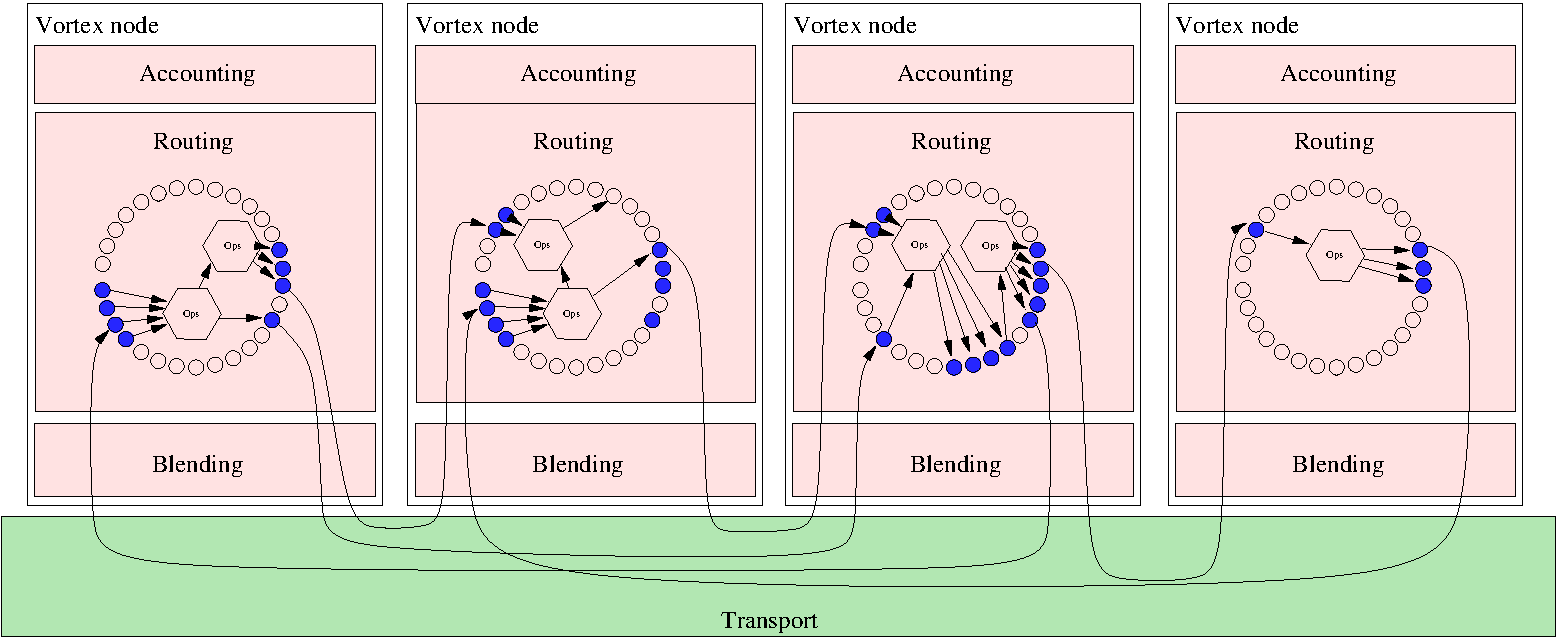
\includegraphics[width=\textwidth]{../../inc/roughProtocolDesign.pdf}
	\caption{A rough protocol outline of the MessageVortex protocol}
	\label{fig:protocolLayers}
\end{figure*}

We were unable to identify a protocol withstanding the strong definition of our adversary. We have, however, found many protocols dealing with anonymity and very few dealing censorship circumventions. We tried to learn from these approaches and tried to integrate useful approaches. It has to be said, however, that very little of the mentioned protocols here had ever experienced broad adoption. Even more, most of them were never implemented or challenged. 

In terms of censorship circumvention, we found that only a little work has been done in academia. Several technical ways have been explored to circumvent censorship. All of them seem to boil down to the following main ideas:
\begin{itemize}
	\item Hide data\\
	The most common approaches we have found were either mimicking protocols (as in \cite{mohajeri2013skypemorph}), use protocols as payload transports (\cite{AthanRAM07}) or employ steganography (as in \cite{f5}) or comparable technologies as side channels.
	\item Copy or distribute data to a vast amount of places in order to improve the lifespan of data\\
	This has been done by systems like \cite{freenet}, or WikiLeaks.
	\item Outcurve censorship measurements\\
	Censorship measurements, especially regarding the Internet censorship of China, have been analyzed in depth under technological, sociological and economical aspects (\cite{Ensafi_2015}, \cite{Clayton_2006}, or \cite{lowe2007great} to name a few)
\end{itemize}

For Anonymization the ideas seem mainly to concentrate around onionizing (ToR\cite{tor-spec}, SOR\cite{Egners_2012}, DUO-Onions and Hydra-Onions\cite{iwanik2005duo}), DC networks (DC-Nets\cite{chaum-dc}, Tarzan\cite{tarzan:ccs02}, GAS\cite{AthanRAM07}), mixing (Babel\cite{babel}, MorphMix\cite{morphmix:wpes2002}, Mixminion\cite{minion-design}, Salsa\cite{Salsa}) and DHT tables (Bifrost\cite{Kondo2009}, BitBlender\cite{Bauer_2008}).

As we use alien transport protocols instead of our protocol, we decided to go for a mixing approach. This approach minimizes the number of messages between the nodes. Furthermore, mixing allows using the nodes in a structureless way as opposed to DC-nets, where we would have to build fixed or ad-hoc rings for exchanging messages. Unlike other protocols, we do not rely on the logic of mixing on the routing node but entirely on the RBB. Routing nodes follow an onionized set of instructions to build messages. 

\section{The MessageVortex Protocol}
In this section, we introduce a new consistent, transport independent model for representing the different protocols used by MessageVortex. The focus of the description lies in academic concepts. For more technical information specifying the protocol as implemented, refer to \cite{MessageVortexRFC}. This document provides details such as specific ASN.1 structures outlining every single block.

\subsection{General Design}

Generally, the Vortex System consists only of nodes, whereas a node may be any system always connected to the Internet. This applies to any device regardless of NAT or similar technologies which usually oppose problems for services. Figure~\ref{fig:protocolLayers} shows a network of four nodes passing messages between them. The transport layer is a common message passing protocol on the Internet. This infrastructure is fixed, within the Internet but not modified for the protocol. It serves as a store-and-forward infrastructure. Although we used SMTP for our experiments, it is not limited to this protocol. The RFC draft document also specifies XMPP. We refer to the red part of each node as VortexNode. These nodes may be any device with a permanent connection to the Internet (e.g., a RaspberryPi computer or a mobile phone).

The Vortex system routes messages from a sender to one or more recipients. We refer to the message sent by the sender and received by the recipients as ``message''. We use the term ``VortexMessage'' for the messages exchanged between the nodes containing either message parts, full messages or decoy traffic.

Each Vortex node constitutes out of three layers. A blending layer embedding and extracting messages from the transport layer, a routing layer processing the VortexMessages and providing ``workspaces'' for ``ephemeral identities'', and an accounting layer authorizing messages. We describe the inner workings of these layer in detail in the next sections.

The protocol handles messages which are passed by a transport protocol from node to node. The instructions how and when to pass a message is generated by a ``routing block builder'' (RBB). The RBB defines the path of the message, the type of hiding (blending) in the transport protocol, and the operations applied to each part of the message in each node. To avoid collision of operations, an RBB has ``ephemeral identities'' on each node with an assigned workspace. Ephemeral identities are short term identities containing a workspace and message quotas for a limited time. Ephemeral identities of a node are unrelated to each other. In the workspaces attached to the ephemeral identities, messages may be assembled, transformed, or decomposed with the operations above. Results are sent to other nodes. Due to the nature of the operations, all messages passed on may be decoy traffic or ``real message parts'' (We prove this claim in section \ref{sec:staticAnalysis}). A node knows that a message is destined for it when a message results in data in specific parts of the identities workspace.

The RBB may be the sender of a block or a different node. If the RBB is not identical to the sender, then the sender is using the routing block for sending a message without knowing its final destination.

\subsubsection{Message Outline\label{sec:messageOutline}}
%%%%%%%%%%%%%%%%%%%%%%%%%%%%%%%%%%%%%%%%%%%%%%%%%%%%%%%%%%%%%%%%%%%%%%%%%%%%%%%%%%%%
%%% Manual float placement
%%%%%%%%%%%%%%%%%%%%%%%%%%%%%%%%%%%%%%%%%%%%%%%%%%%%%%%%%%%%%%%%%%%%%%%%%%%%%%%%%%%%
\begin{figure*}[ht]
	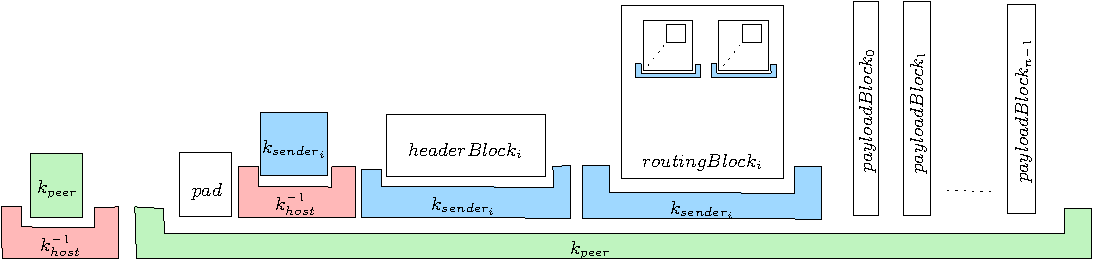
\includegraphics[width=\textwidth]{../../inc/blockLayoutSimplified}
	\caption{Simplified message outline}
	\label{fig:messageOutline}
\end{figure*}

We show in Figure~\ref{fig:messageOutline} a simplified view on a VortexMessage.

A VortexMessage is passed from one router to another and is embedded as binary data in the transfer protocol. Every Vortex node may decide for himself on the support of algorithms and embedding mechanisms.

The block structure of a Vortex message is as follows:
\begin{itemize}
	\item Encrypted peer key $k_{peer_n}$\\
	Contains symmetrical key for decryption of follow up header information and payload blocks. The key is encrypted with the receiving host's public key. The key is known to the RBB, the message sending node, and the message receiving node. No other node knows the key.
	\item padding\\
	This padding makes sure that the message part encrypted with the peer key does look different for each payload even when reusing keys. This case is not recommended but unavoidable in the case of a reused routing block. Using a different IV, in this case, is not an option as the IV is specified in the routing block and thus replayed as well.
	\item header block encrypted with $k_{sender_n}$ and signed with the identities private key (detached signature).
	\begin{itemize}
		\item Identity and ``proof of work'' information\\
		This information contains the public key of the identity. It serves as an identifier for the workspace and is authenticates by the signature.
		\item Replay protection information\\
		This information allows a node to identify replayed Messages even if the payload of the content has been modified.
		\item Forward secret information\\
		This information allows a node to identify VortexMessages where tampering occurred by recombining blocks of multiple messages.      
		\item (optionally) Proof-of-work information\\
		This information allows a sending node to fulfill a proof of work requirement raised due to a previously sent request.      
	\end{itemize}
	\item Routing blocks (encrypted with sender key)
	\begin{itemize}
		\item Next hop timing instructions
		This specifies by when building instructions should be carried out relative to the moment of reception of the VortexMessage. It is specified as a time range. There may be multiple timing instructions. Each of the instructions refers to precisely one routing block and one header block.
		\item Next-hop routing blocks\\
		These routing blocks are placed into the VortexMessage created according to the build instructions and are already encrypted with $k_{sender_{n+1}}$ and thus not readable to the current node.
		\item Next hop header (encrypted with $k_{sender_{n+1}}$)
		These header blocks are placed into the VortexMessage created according to the build instructions and are already encrypted with $k_{sender_{n+1}}$ and thus not readable to the current node.
		\item Message build instructions.\\
		These instructions form the core for the workspace and contain all instructions and the information which payload blocks should be included in each of the messages.
		\item Next hop peer key $k_{peer_{n+1}}$.\\
		This part may contain one or more peer keys.
		\item Next hop blending instructions.\\
		These contain the information about what transport to use, what blending to use, and the address of the next router node.
	\end{itemize}
	\item Encrypted payload blocks (encrypted with peer key)
	\begin{itemize}
		\item Payload blocks
	\end{itemize}
\end{itemize}

It is important to note that there are two symmetrical keys involved in encrypting and decrypting message headers. Having two keys is not a flaw in the protocol but necessary. 

The first key of a VortexMessage is the peer key $k_{sender_n}$. This key is only accessible with the private key of the node receiving the message and is furthermore known by the RBB. It allows decryption of the routing blocks concerning the current node and the header information. The sender of a message block is therefore not able to tell if a VortexMessage contains one or more routing blocks for the next node. It is important to note that no other node should have access to this information as this builds the unlinkability between two non-adjacent nodes. 

The second key is the peer key $k_{peer_n}$ located in the encrypted header. The RBB chooses the key. This key protects the inner structure of the message. It makes it impossible for any node except the sending or the receiving peer node to detect the inner structure of the message. Without this key, any independent observer with knowledge about the blending capabilities of a receiving node may:
\begin{itemize}
	\item easier identify the block structure.\\ 
	This remains the case regardless of whether ASN.1 or length prefixed structures are used. If the structure of a vortex Message is identifiable, the messages may be logged or dropped by an adversary.
	\item Identify the routing block size.\\
	The value of this information is only minimal as it only reflects the complexity of the remaining routing information indirectly.
	\item Identify the number of payload blocks and their respective sizes. \\
	This is valuable information when following the traffic of a message.
\end{itemize}

Furthermore, by providing a pre-encrypted key, we hide the asymmetric key required to the next node. So, a node can compile a message for another node without being aware of the required public key.

\subsubsection{Accounting Layer}
The Accounting layer maintains all local identities called ephemeral identities and controls the overall load to the system. Ephemeral identities are temporary accounting objects identified with the public part of an asymmetric key. 

The accounting layer processes requests from other nodes. Each request is either a request for information about the node, the creation of a new ephemeral identity, or a request to process messages. The accounting layer creates replies to such requests and maintains the accounting information of such an entity. The accounting layer has the options to either accept a request, reject a request, silently drop a request (usually done to improve privacy), or to request the solving of a proof-of-work puzzle (puzzle). To send a reply to the unknown requester, the header block contains a routing block prebuilt by the RBB.

The only implemented puzzle so far is a hash-based puzzle. The puzzle opposes that a header block $\mathbf{H_{t-1}}$ has to be resent including a challenge $c$ (an ASN.1 octet string) and has to result in a specific bit sequence $s$ of the hashed block with signature.

Therefore we assume that a validly solved puzzle when:

\begin{eqnarray}
\mathbf{HEADER} & = &D^{K_{sender}}\left(\mathbf{H}\right) \\
& = &\langle H_{t-1}, c\rangle\\
puzzleSolved    & = &H_{spec}(\mathbf{H}).startsWith(s)
\end{eqnarray}

The puzzle has an assigned lifetime. To solve the puzzle successfully, the requesting host has to solve this puzzle within the specified time frame. 

\subsubsection{Routing Layer}
The routing layer processes the messages. Incoming messages are passed after extraction by the blending layer to the routing layer. There the message is disassembled in its components.

As operations, we use some general capabilities such as splitting a message into two payload blocks and merging them again. Another type of operation is encryption and decryption of payload blocks. The third and most important type of operation is a redundancy operation. This operation uses a Reed-Solomon\cite{reed1960polynomial} function to add redundancy information to the data while obfuscating its content. This function has previously been proposed mainly for information sharing systems (e.g., \cite{mceliece1981sharing}).

A routing block may be used once or multiple times if flagged accordingly. Repeating a routing block allows a sender to use a routing block as an anonymous endpoint address. It is essential to understand that reusing a routing block does have downsides in terms of privacy. Reusing a routing block does typically create the same pattern on the network assuming the same workspace layout. While the timing might vary the number of messages and the sequence of messages remains the same. For a full list of weaknesses when reusing routing blocks, see \ref{sec:dynamicAnalysis}.

Tasks of the routing layer are:
\begin{itemize}
	\item Build structure representing the block building and the appropriate block IDs.
	\item Schedule all Routing blocks for processing in a priority queue.
	\item Authorize all routing blocks ready for processing with the calculated block sizes.
	\item Process blocks.
	\item Send prepared building blocks to the Blending layer.
\end{itemize}

The workspace of an ephemeral identity is Shown in Figure~\ref{fig:workspace}.

\begin{figure}[ht]
	\centering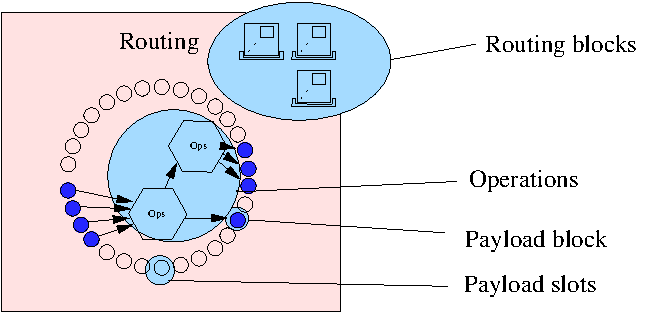
\includegraphics[width=\columnwidth]{../../inc/roughProtocolDesign_workspace.pdf}
	\caption{Layout of a workspace}
	\label{fig:workspace}
\end{figure}

Each workspace stores objects for a limited amount of time. 

\subsubsection{Blending Layer}
The blending layer provides the ``undetectability'' feature of the Vortex system. To avoid transport protocol misuse and unintentional exit nodes of the protocol, the RBB has no control over the transported content except for the hidden VortexMessage and how it is embedded. This rule loads the burden of sensible cleartext payload generation to the blending layer. 

A blending layer may provide multiple strategies to embed a message. In our prototype, we always sent a VortexMessage by embedding its content into an attachment. While F5\cite{f5} is currently preferred for embedding, current implementation supports as well so-called plain embedding simply replacing the file content of the attachment with the VortexMessage. This may be done starting at character 0 or any offset supported by the blending layer (to leave header data intact).

Furthermore, this layer is taking care of multiple problems:
\begin{itemize}
	\item Translating the message into the transport format\\
	This translation includes jobs such as embedding a message as encoded text, as a binary attachment or hide it within a message using steganography.
	\item Extract incoming messages from the transport protocol\\
	Identify incoming messages containing a possible block and extract it from the message.
	\item Do housekeeping on the storage layer\\
	Access protocols such as POP and IMAP require message deletion after processing to stay below the sizing quotas of an account.         
\end{itemize}

We define the blending layer to work as follows when receiving messages:
\begin{enumerate}
	\item Log arrival time (in UTC) on the transport layer.
	\item Extract possible blocks.
	\item Apply decryption on a suspected header block.
	\item Validate the header block using the accounting layer.
	\item Process header requests (if any)
	\item Extract and decrypt subsequent blocks.
	\item Pass extracted blocks and information to the routing layer.
\end{enumerate}

We define the blending layer to work as follows for sending messages:
\begin{enumerate}
	\item Assemble message as passed on by the routing layer.
	\item Using the blending method specified in the routing block build an empty message. 
	\item Create a message body content.
	\item Send the message to the appropriate recipient using the transport layer protocol.
\end{enumerate}

For our first tests, we used a custom transport layer, allowing us to monitor all traffic quickly, and build structures in a very flexible way. This transport layer works locally with a minimum amount of work for setup and deployment. It furthermore works across multiple hosts in a broadcast domain. The API may be used to support almost any kind of transport layer. After that, we focused on the protocols identified as suitable as transport protocols:
\begin{itemize}
	\item SMTP
	\item XMPP
\end{itemize}
For the prototype, we have implemented an SMTP transport agent and the respective blending layer.

The routing layer receives the message blocks in a decrypted and authorized form from the blending layer. The routing layer then assembles all information of an identity and makes executes the accepted operations using the available data. 

It is relatively easy to generate a credible cleartext message to pass an automated testing engine. This statement may be verified by looking at the effectivity of today's junk mail filters. These filters have huge problems continuously adapting to the new types of unsolicited bulk emails (UBE).

Things do, however, drastically change if taking a human censor into account. A human censor is not only able to analyze the text and layout of a message. He is furthermore capable of judging on the stringency of a communication. He may deduce data such as relationship and type of writing. Then, he may detect anomalies within conversations and judge whether the communication pattern is more likely to be from a human or a chatbot.

\subsubsection{Applied Steganography and the Dead Parrot}
A human censor can take very complex information into account when it comes to analyses of message content. He is not only able to analyze a message for its content, but he may also see the message in the context of other messages. In \cite{oakland2013-parrot} is expressed that it is easy for a human to determine decoy traffic as the content is easily identifiable as generated content. While this is true for the very general case, there is a possibility here to generate ``human-like'' data traffic to a certain extent. As an adversary may not assume that his messages are replied to, the problem does not boil down to a Turing test. It remains on the level of a ``passive observer Turing test'', in this scenario the censor is only able to judge on the given messages instead of introducing his own questions, wordings, and verbal challenges. By enabling the potential nodes to choose their messages and the replies generated to them, we enabled them to choose very reduced types of communications. The chosen messages may even be identifiable as automated messages (e.g., messages of a monitoring system or messages of an SMS to email gateway). 

The most straightforward approach would have been to give a routing block builder the means of controlling the decoy message content. While such a possibility would be easy, it would enable a routing block builder to use the node as a ``exit node'' from the system. Blackmailing messages could be sent through the system to a non-participating member and leak at the same time the presence of a routing node. To deny this possibility, we shifted the ability to the routing node.

The VortexMessage itself is binary, and as such, there are only limited possibilities to hide it within the transport protocol. We decided to use attachments or attachment-like structures. Within the attachments, we currently support two types of embedding: plain and steganographic embedding. 

Plain embedding means that we insert a sequence of blocks into a standard message. This is typically done within files with a weaker structure and high entropy (such as an MP3 encoded file). While this is very hard to detect for a machine, it becomes immediately suspicious for a human censor. A human censor would detect the presence of a payload which does not make any sense.

For steganographic embedding, we decided to go for F5\cite{f5}. It is a reasonably well-researched algorithm which attracted many researchers. The original F5 implementation had a detectable issue with artifacts\cite{F5broken} caused by the recompression of the image. This issue was caused only due to an issue in the reference implementation, and the researchers have provided a corrected reference implementation without the weakness. Like always, the type of embedding may be specified and replaced upon request. 

\subsection{The Core: Operations}
We differentiate three types of operations:
\begin{itemize}
	\item Splitting and merging of chunks
	\item Encryption and decryption of chunks
	\item Redundancy calculations carried out on chunks
\end{itemize}

The first two Operations do not provide a high level of unlinkability as they do allow analysis such as hotspot analysis and produce continuously inclining, steady or declining message sizes depending on the type of use. The third operation, however, adds a whole lot of new possibilities in conjunction with the other two.

\subsubsection{Splitting and Merging}
The splitPayload operation splits a payload block into two chunks of different or equal sizes. The parameters for this operation are:

\begin{itemize}
	\item source payload block $pb_1$
	\item fraction $f$\\
	A floating-point number which is describing the size of the first chunk. If the fraction is ``1.0'', then the whole payload is transferred to the second target chunk
\end{itemize}

If $len(pb_1)$ expresses the size of a payload block called $pb_1$ in bytes, then the two resulting blocks of the SpitPayload Operation $pb_2$ and $pb_3$ have to follow the following rules:

\begin{eqnarray}
split(f, pb_1) & = &\langle pb_1, pb_2 \rangle\\
pb_1.startsWith(pb_2)\\
pb_1.endsWith(pb_3)\\
len(pb_2) & = & \lfloor len(pb_1)\cdot f\rfloor\\
len(pb_1) & = & len(pb_2) + len(pb_3)
\end{eqnarray}

The mergePayload operation combines two payload blocks into one. The parameters for this operation are:

\begin{itemize}
	\item first source payload block $pb_1$
	\item second source payload block $pb_2$
\end{itemize}

If $len(pb)$ expresses the size of a payload block called $pb$ in bytes then resulting block of the MergePayload Operation $pb_3$ have to follow the following rules:

\begin{eqnarray}
merge(pb_1, pb_2) & = & pb_3 \\
pb_3.startsWith(pb_1)\\
pb_3.endsWith(pb_2)\\
len(pb_3) & = & len(pb_1) + len(pb_2)
\end{eqnarray}

\subsubsection{Encryption and Decryption}
The encryptPayload operation encrypts a payload block $pb_1$ symmetrically resulting in a block $pb_2$. The length of block $pb_2$ may vary according to mode and padding chosen. The parameters for this operation are:

\begin{itemize}
	\item Source payload block $pb_1$
	\item Encryption specification $spec$
	\item Symmetric key $k$
\end{itemize}

The operation follows the following rules (please note section \ref{sec:encNot} for notation):
\begin{eqnarray}
encrypt(pb_1, spec, K_a) & = & pb_2 \\
pb_2 & = & E_{spec}^{K_a}\left( pb_1 \right)\\\
len(pb_2) & \geq & len(pb_1)
\end{eqnarray}


The decryptPayload operation decrypts a payload block $pb_1$ symmetrically resulting in a block $pb_2$. The length of block $pb_2$ may vary according to mode and padding chosen. The parameters for this operation are:

\begin{itemize}
	\item Source payload block $pb_1$
	\item Decryption specification $spec$
	\item Symmetric key $k$
\end{itemize}

The operation follows the following rules (please note section \ref{sec:encNot} for notation):
\begin{eqnarray}
decrypt(pb_1, spec, K_a) & = & pb_2 \\
pb_2 & = & D_{spec}^{K_a}\left( pb_1 \right)\\
len(pb_2) & \leq & len(pb_1)
\end{eqnarray}

\subsubsection{Redundancy Operations}
These operations build the core of the mixing operations. The operation allows to add to a message redundancy information or to rebuild a block from a chosen set of information. 

The operation itself is shown in Fig.~\ref{fig:addRedundancyOperation}. 
\begin{figure}[ht]\centering
	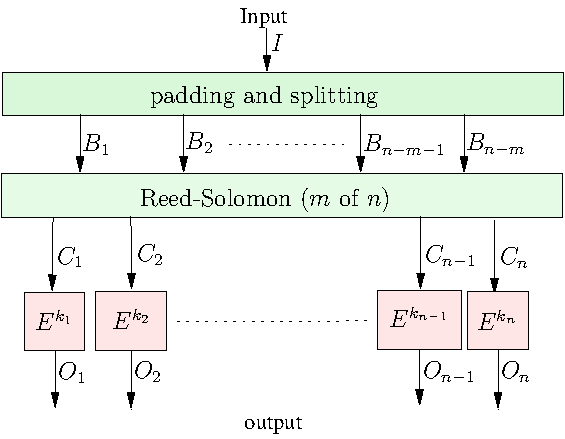
\includegraphics[width=0.8\columnwidth]{../../inc/addRedundancyOp}
	\caption{Outline of the addRedundancy operation}
	\label{fig:addRedundancyOperation}
\end{figure}

It may be subdivided into the following operations:
\begin{itemize}
	\item Pad the original message block in such a way, that all resulting blocks are a multiple of the block size of the encrypting cipher.
	\item Apply a Reed-Solomon operation in a given GF space with a Vandermonde matrix.
	\item Encrypt all resulting blocks with unpadded, symmetrical encryption.
\end{itemize}

The padding is not standard padding from encryption. The reason for this lies in the properties required in the padding. These properties were:
\begin{itemize}
	\item The padding must not leak whether the rebuild cycle was successful or not.
	\item The padding should not leak whether a removeRedundancy operation was successful or not. 
	\item Anyone knowing the routing block content and the transmitted message must be able to predict any treated block including all padding bytes.
	\item The padding must work with any size padding space.
\end{itemize}

The padded block $\mathbf{X}$ is created from a padding value $p$, the unpadded block $\mathbf{M}$ and a srie of padding bytes. We build $\mathbf{X}$ for a function $RS_{\text{m of n}}$ and an encryption block $\mathbf{M}$ sized $k$ as follows:
\begin{eqnarray}
i          & = & len(\mathbf{M})\\
e          & = & k \cdot n\\
l          & = & \left\lceil\frac{i + 4 + C2 }{e}\right\rceil\cdot e\\
p          & = & i + \left( C1 \cdot l \pmod{\left\lfloor\frac{2^{32}-i}{l}\right\rfloor\cdot l}\right)\\
\mathbf{X} & = & \langle p,\mathbf{M},R_{t}\left(s,l-i-4\right)\rangle
\end{eqnarray}    
The remainder of the input block, up to length $l$, is padded with random data. The random padding data may be specified by RBB though a PRNG spec $t$ and an initial seed value $s$. The message is padded up to size $L$. All resulting, encrypted blocks do not require any padding. This baecause the initial padding guarantees that all resulting blocks are dividable by the block size of the encrypting function. If not provided by an RBB, an additional parameter $C1$ is chosen as random positive integer and $C2=0$  by the node executing the operation.

To reverse a successful message recovery information the of a padded block $\mathbf{X}$, we calculate the original message size by extracting $p$ and doing $len(\mathbf{M})=p \pmod{ len(\mathbf{X})}$.

This padding has many important advantages:
\begin{enumerate}
	\item The padding does not leak if the rebuilding of the original message was successful. Any value in the padding may reflect a valid value.
	\item Since we have a value $C2$, the statement that a message size is within $len(\mathbf{X})<size<(len(\mathbf{X})-k\cdot n)$ is no longer true and any value smaller $len(\mathbf{X})-k\cdot n$ may be correct as well.
	\item An RBB may predict the exact binary image of the padded message when specifying $C1$, $C2$, and $R_{t}(s,)$.
\end{enumerate}

The Reed-Solomon operation is done with a Vandermonde matrix. Unlike in error correcting systems, we do not normalize the matrix so that the result of the first blocks is equivalent to the original message. Instead, the error correcting information is equally distributed over all resulting blocks adding further obfuscation. Since the entropy of the resulting blocks is lowered and may thus leak an estimate of how a resulting block may have been treated, we added the encryption step to equalize entropy again. The previously introduced padding guarantees that there is no further padding on block level required. Such padding could leak in case of decryption whether the block has been altered or not.

\subsection{Usage of the Protocol}
First, a sending node collects either a set of nodes and keys it wants to use and creates identities on these nodes using header requests. Then the sender creates a routing block containing all the routing instructions (hops and operations). Alternatively, a sender may use a premanufactured routing block for the specified target. This routing block is then concatenated to a message and passed to the locally running routing node. From there the message is routed as defined in the routing block. An example of such a route is shown in Figure~\ref{fig:protocolLayers}.

A trivial routing block may only include the direct hop from the sender to the receiver. When adding subsequent decoy paths leaving the receiver, it is even for an adversary capable of mapping ephemeral identities to the respective RBB impossible to tell the final recipient. This since a message may increase or decrease in its size even after the final delivery through the addRedundancy operation. Even the recipient node is unable to tell if there are any other messages routed if appropriately crafted.

If a node is always using a set of $k$ recipients of its address book, at least $k$ anonymity is achieved. If an adversary compromises all other nodes involved in routing, he is still unable to tell anything

\section{Discussion of the Results}
We first focus on the protocol itself to show the strength an weaknesses of the protocol. After that, we focus on the dynamic part and see what type of data may be collected when considering not only the protocol but the whole message flow. We then present guidelines for different jurisdictional types.

We focus on an adversary in an environment, where the participation as a MessageVortex router, is considered a criminal act and highlight some additional constraints applying in such situations.

\subsection{Static Protocol Analysis\label{sec:staticAnalysis}}
A VortexMessage is not identifiable as the message is structureless on the outside. The VortexMessage itself follows the encrypted key without any structure. Therefore, we require the hosts private key to tell whether there is VortexMessage within a transport message or not.

The communication itself is undetectable for an adversary only observing as long as the blending mechanism is secure, and the plain text communication of a node does not differ from any other communication. While we can monitor the first criteria, the latter is far harder to achieve or measure as it involves many unobvious properties. Obvious properties are the credibility of message content or stringency of communication over all messages. Unobvious properties may be the frequency of messages (e.g., bundling of messages showing an inappropriate speed of writing to a single entity or 24x7 activity of a natural person) or a message exchange massively in favor of one recipient. We were not able to create a set of measurable properties covering these properties.

The padding block $PAD$ makes sure that, even if a routing block is reused, the VortexMessage structure is not the same. However, the preceding block with the key remains the same unless the RBB provided multiple key blocks. If a key block is reused, an adversary to identify repeated MURBs by this fingerprint.

Next, and one of the biggest problems we found is that a VortexNode is aware of its immediate peers. This flaw is because we do require a routable address for the transport protocol. Vortex nodes may thus discover their immediate peers. It is, on the other side, not possible to use discovered peers. To use a peer, a transport address and a host key are required. A VortexNode may query this key, but there is no obligation to reply for the node asked for the key. We were unable to find a protocol commonly used on the Internet, allowing to cloak the receiving node of a message.

An active adversary may not create its routing blocks or header blocks and inject them due to the forward secret. He may, however, replace the peer key of a message. As this key is known to him, he gains no additional knowledge. Replacing the sender key block breaks the message. Replacing the header or routing block of the message with another header or routing block from the same ephemeral identity breaks the message unless the RBB reused the sender key and the forward secret. Finally, exchanging, omitting, or adding payload blocks renders the message inoperable, but does not generate additional knowledge. Replying the same or a modified block does not generate any pattern on the network as the replay protection stops propagating messages at the next node. Thus, a replayed block does not generate new knowledge to an observer.

All operations may apply to true message chunks as well as decoy traffic. As a node cannot tell if a traffic arriving is a decoy or true message content, it is unable to tell apart what outgoing traffic is a decoy. An encrypted block is of the same nature before and after encryption. As we do not know the blocks nature before, we are unable to tell the blocks nature after the encryption. The same argument applies to decryption, split, and merge operations. 

Redundancy operations are alike. They, however, fulfill an additional purpose. A $addRedundancy$ operation adds size to a message without differentiating between redundancy information and original payload. If the original block was a decoy, then all resulting blocks are decoys. If an originating block was message content, then all resulting blocks hold the same amount of data from the original block. So, this operation allows decoy traffic generation without enabling a generating node to identify the decoy traffic.

\subsubsection{Endpoint Operation}
Depending on the blending method, an adversary may identify single messages as long as they are detectable. Detectability depends on various factors, such as:
\begin{itemize}
	\item Broken internal file structure (due to plain blending)
	\item Uncommon high entropy in a structureless file
	\item Unrelated message flow (see \cite{oakland2013-parrot})
	\item Non-human behavior on the transport layer (e.g., message traffic 24x7)
\end{itemize}

If an adversary identifies an endpoint successfully, then all peering endpoints of the same protocol may be identified as well by following the message flow. This does, however, not enable an adversary to inject messages as the host key is not known. 

Assuming a global observer as an adversary and unencrypted traffic, he might discover the originating routing layer and thus identify it as Vortex node by following traces of the transport layer. In most protocols, however, this address is spoofable and not a reliable source for the originating account.

\subsubsection{Conclusions Based on Ephemeral Identities}
The knowledge a node may gain from ephemeral identities is minimal. The ephemeral identity is created by a node unknown to the receiver of the request. The only thing we know is what node was adjacent when creating the ephemeral identity. As the creation of an ephemeral identity is not linked to any other identity or ephemeral identity relationship between ephemeral identities on two nodes cannot be established. If two adjacent nodes cooperate when processing two linked ephemeral identities, no additional knowledge may be won. If two collaborating nodes have one or more non-collaborating nodes between them, they lose all linking knowledge due to the non-collaborating nodes. 

\subsubsection{Conclusions from Operations}
Operations have been carefully crafted to leak as little information as possible. Being able to encrypt or decrypt a payload block does not leak any information. The data processed may be true message traffic or decoy as we do not know what the nature of the received message was. If an RBB avoids repeating patterns on nodes, it is not possible to link ephemeral identities of two non-adjacent nodes. Repeating patterns may arise, for example, if a block $pb_1$ is decrypted and re-encrypted on two nodes. In this case, both nodes may match the message as it contains the same content between the operations.

\begin{eqnarray*}
	\text{node f:}\\
	& pb_2 & = D(pb_1)\\
	& pb_3 & = E^{K_t}(pb_2)\\
	\text{node f+1:}\\
	&.\\
	&.\\    
	\text{node f+x:}\\
	& pb_4 & = D^{K_t}(pb_3)\\
\end{eqnarray*}

In this example the patterns of $pb3$ and $pb_4=pb_2$ are two patterns repeating on non-adjacent nodes. The same conclusions are even more valid for splitting operations. These two operations should be regarded as helpers for the $addRedundancy$ and $removeRedundancy$ operations. These operations may be used to generate decoy traffic or to destroy data without knowledge of doing so of the processing node. If we process a function $addRedundancy_{2 of 3}$ any of the output blocks contains the input payload and any two of them may be used to recover the data. At the same time, an operation $removeRedundancy_{2 of 3}$ may be successful or not. The node is unable to differentiate between the two states. The padding applied and the unpadded encryption makes it impossible to judge upon success or fail of an operation.

\subsection{Dynamic Protocol Analysis\label{sec:dynamicAnalysis}}
A global observer is unable to analyze a message flow by timing or pattern of the exchanged packet even when being able to identify message vortex packages. Entry and exit nodes are indistinguishable even if having infiltrated significant portions of the network. Cooperation between adjacent nodes does not gain more information as all operations are minimized then to one combined workspace with all the operations. Linking of the message of two non-adjacent nodes is not possible as there are no linking attributes.

\subsubsection{Bootstrapping of Addresses and Identities}
Using the header requests an adversary may discover nodes over time. While it is not possible to screen traffic destined to such nodes, a global observer may identify peer partners of these nodes on the transport level.

\subsubsection{Discovery of Peer Nodes}
Besides attacking the message content, attacking the routing nodes is an option for an adversary in a jurisdiction where the operation of such a node is a criminal act. The presence of routing nodes is valuable information for a global observer narrowing down the information regarding data to be analyzed.

\subsubsection{Findings based on Adversary Environment}
In environments containing only global observers and no jurisdictional constraints regarding the technology, a VortexNode may disclose its presence. This means a VortexNode is not forced to cloak its presence. In such an environment, an RBB should choose the operations to be sensible, but great care is not required. Even if there is a node with a known owner of the node and a suspected message is received, the owner may credibly claim that the message in question was a decoy. No information obtained by any node involved in the routing of the message may proof anything else. Since a message may be split into any number of parts and related messages are only identifiable with a high degree of improbability even meta information such as the real size of the message, the sending time or the involved parties in the anonymity set are unknown. This statement is still valid if we consider an active adversary.

In environments where using a VortexNode is subject to criminal prosecution, much more care has to be applied. As all routing nodes know their immediate peer, we were only able to find two weak solutions to this problem. The first solution is only to use trusted nodes. If we can trust all routing nodes, no external observer may prove that the message flow is, in fact, MessageVortex traffic. An adversary node within such a system can learn the addresses of other nodes within the set. The RBB may reduce the set of uncovered nodes by applying communicating groups of nodes (communication cells) with defined gateways nodes between them. In such a scenario, only a cell and a possible adjacent cell may be discovered.

\subsubsection{Issues When Reusing Routing Blocks}
Reusing a routing block is required if the receiver is not known, and a continuous stream of messages is required. Although it is possible to use multiple single route routing blocks (SURB) instead of one multi-use routing block (MURB), it is costly. These costs arise due to the necessary calculation power to create identities. MURBs do have, however, significant drawbacks in terms of unlinkability and should be, therefore, avoided if possible.

A MURB creates a repeated pattern on the network in terms of messages. For a routing node, it is evident that the same tuple of communication partners is exchanging messages. The size of the VortexMessage allows in such a case an estimate of the current size in relation to the previous messages.

Furthermore, security is affected when using MURBs. A MURB may be replayed and allows thus to exhaust quotas of an ephemeral identity. To counter such exhaustion, the protocol introduces a maximum replay rate, but this is only weak protection.

\section{Conclusion}
Creating a protocol which is possibly censorship resistant, is already hard. The analysis showed that even when a protocol is crafted with great care, braking unobservability is far simpler than doing it right. MessageVortex does show the desired properties. The protocol allows sending a message from a sender to a recipient without exposing the linking between the two. Traditional analysis, such as hotspot analysis, fail since the operations successfully hide properties of the message flow. At the same time, we were able to present a system which requires an unmatched amount of observation, infrastructure, and calculation power to be broken.

\subsection{The Missing Links and Future Research}
A lot still needs to be done. For this protocol to be of any use, a user-friendly implementation is required. The currently released implementation works as a prototype for academic research. It is, however, far beyond from being user-friendly. Too many choices are currently left to the user. A new implementation must provide excellent censorship resistance while providing easy to use recipes for message transfer.  

For the traffic to be truly undetectable, chatbots must generate meaningful conversation between blending nodes. This conversation does not necessarily boil down to a Turing test. It is sufficient that two blending layers are capable of setting up communication, which is indistinguishable from a regular human or machine communication. As an adversary is typically not able to generate own traffic without exposing the probing activity and a blender is not required to such probes, an attacker is very limited.

Furthermore, some issues have been identified, relating to updating nodes. A node should be able to request the software over VortexMessages as official sources for updates may be blocked. 

Next is the problem of the routing node. The hardware of such a node should be protected with a small platform featuring deniable encryption and anti-forensic measures. We are currently investigating the possibility of creating such a cheap platform based on a RaspberryPi Zero.

Another exciting field of academic research is creating strategies for Routing block builders (RBB). We currently have a toolset of powerful operations, but academic researched strategies or guidelines for good routing blocks are missing. 

\hfill gwm
 
\hfill May 8, 2019

%\subsection{Subsection Heading Here}
%Subsection text here.

% needed in second column of first page if using \IEEEpubid
%\IEEEpubidadjcol

%\subsubsection{Subsubsection Heading Here}
%Subsubsection text here.


% An example of a floating figure using the graphicx package.
% Note that \label must occur AFTER (or within) \caption.
% For figures, \caption should occur after the \includegraphics.
% Note that IEEEtran v1.7 and later has special internal code that
% is designed to preserve the operation of \label within \caption
% even when the captionsoff option is in effect. However, because
% of issues like this, it may be the safest practice to put all your
% \label just after \caption rather than within \caption{}.
%
% Reminder: the "draftcls" or "draftclsnofoot", not "draft", class
% option should be used if it is desired that the figures are to be
% displayed while in draft mode.
%
%\begin{figure}[!t]
%\centering
%\includegraphics[width=2.5in]{myfigure}
% where an .eps filename suffix will be assumed under latex, 
% and a .pdf suffix will be assumed for pdflatex; or what has been declared
% via \DeclareGraphicsExtensions.
%\caption{Simulation results for the network.}
%\label{fig_sim}
%\end{figure}

% Note that the IEEE typically puts floats only at the top, even when this
% results in a large percentage of a column being occupied by floats.
% However, the Computer Society has been known to put floats at the bottom.


% An example of a double column floating figure using two subfigures.
% (The subfig.sty package must be loaded for this to work.)
% The subfigure \label commands are set within each subfloat command,
% and the \label for the overall figure must come after \caption.
% \hfil is used as a separator to get equal spacing.
% Watch out that the combined width of all the subfigures on a 
% line do not exceed the text width or a line break will occur.
%
%\begin{figure*}[!t]
%\centering
%\subfloat[Case I]{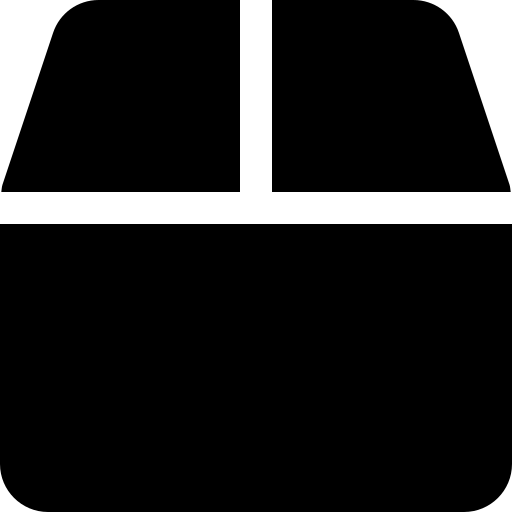
\includegraphics[width=2.5in]{box}%
%\label{fig_first_case}}
%\hfil
%\subfloat[Case II]{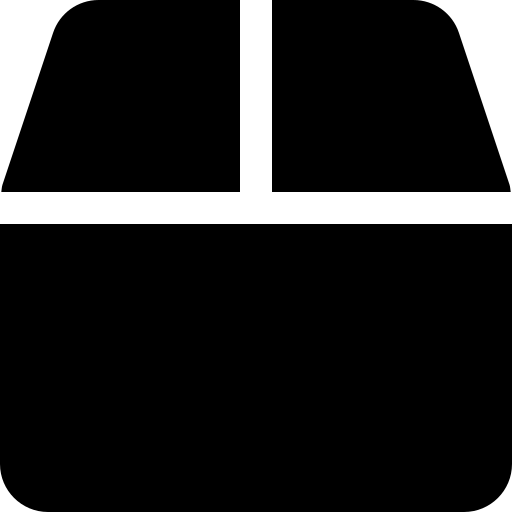
\includegraphics[width=2.5in]{box}%
%\label{fig_second_case}}
%\caption{Simulation results for the network.}
%\label{fig_sim}
%\end{figure*}
%
% Note that often IEEE papers with subfigures do not employ subfigure
% captions (using the optional argument to \subfloat[]), but instead will
% reference/describe all of them (a), (b), etc., within the main caption.
% Be aware that for subfig.sty to generate the (a), (b), etc., subfigure
% labels, the optional argument to \subfloat must be present. If a
% subcaption is not desired, just leave its contents blank,
% e.g., \subfloat[].


% An example of a floating table. Note that, for IEEE style tables, the
% \caption command should come BEFORE the table and, given that table
% captions serve much like titles, are usually capitalized except for words
% such as a, an, and, as, at, but, by, for, in, nor, of, on, or, the, to
% and up, which are usually not capitalized unless they are the first or
% last word of the caption. Table text will default to \footnotesize as
% the IEEE normally uses this smaller font for tables.
% The \label must come after \caption as always.
%
%\begin{table}[!t]
%% increase table row spacing, adjust to taste
%\renewcommand{\arraystretch}{1.3}
% if using array.sty, it might be a good idea to tweak the value of
% \extrarowheight as needed to properly center the text within the cells
%\caption{An Example of a Table}
%\label{table_example}
%\centering
%% Some packages, such as MDW tools, offer better commands for making tables
%% than the plain LaTeX2e tabular which is used here.
%\begin{tabular}{|c||c|}
%\hline
%One & Two\\
%\hline
%Three & Four\\
%\hline
%\end{tabular}
%\end{table}


% Note that the IEEE does not put floats in the very first column
% - or typically anywhere on the first page for that matter. Also,
% in-text middle ("here") positioning is typically not used, but it
% is allowed and encouraged for Computer Society conferences (but
% not Computer Society journals). Most IEEE journals/conferences use
% top floats exclusively. 
% Note that, LaTeX2e, unlike IEEE journals/conferences, places
% footnotes above bottom floats. This can be corrected via the
% \fnbelowfloat command of the stfloats package.




%\section{Conclusion}
%The conclusion goes here.





% if have a single appendix:
%\appendix[Proof of the Zonklar Equations]
% or
%\appendix  % for no appendix heading
% do not use \section anymore after \appendix, only \section*
% is possibly needed

% use appendices with more than one appendix
% then use \section to start each appendix
% you must declare a \section before using any
% \subsection or using \label (\appendices by itself
% starts a section numbered zero.)
%


\appendices
%\section{Proof of the First Zonklar Equation}
%Appendix one text goes here.

% you can choose not to have a title for an appendix
% if you want by leaving the argument blank
%\section{}
%Appendix two text goes here.


% use section* for acknowledgment
%\ifCLASSOPTIONcompsoc
%  % The Computer Society usually uses the plural form
%  \section*{Acknowledgments}
%\else
%  % regular IEEE prefers the singular form
%  \section*{Acknowledgment}
%\fi
%
%
%The authors would like to thank...


% Can use something like this to put references on a page
% by themselves when using endfloat and the captionsoff option.
\ifCLASSOPTIONcaptionsoff
  \newpage
\fi



% trigger a \newpage just before the given reference
% number - used to balance the columns on the last page
% adjust value as needed - may need to be readjusted if
% the document is modified later
%\IEEEtriggeratref{8}
% The "triggered" command can be changed if desired:
%\IEEEtriggercmd{\enlargethispage{-5in}}

% references section

% can use a bibliography generated by BibTeX as a .bbl file
% BibTeX documentation can be easily obtained at:
% http://mirror.ctan.org/biblio/bibtex/contrib/doc/
% The IEEEtran BibTeX style support page is at:
% http://www.michaelshell.org/tex/ieeetran/bibtex/
\bibliographystyle{IEEEtran}
% argument is your BibTeX string definitions and bibliography database(s)
%\bibliography{IEEEabrv,../bib/paper}
%
% <OR> manually copy in the resultant .bbl file
% set second argument of \begin to the number of references
% (used to reserve space for the reference number labels box)
%\begin{thebibliography}{1}
%
%
%\end{thebibliography}
\bibliography{../../messageVortex}

% biography section
% 
% If you have an EPS/PDF photo (graphicx package needed) extra braces are
% needed around the contents of the optional argument to biography to prevent
% the LaTeX parser from getting confused when it sees the complicated
% \includegraphics command within an optional argument. (You could create
% your own custom macro containing the \includegraphics command to make things
% simpler here.)
%\begin{IEEEbiography}[{\includegraphics[width=1in,height=1.25in,clip,keepaspectratio]{mshell}}]{Michael Shell}
% or if you just want to reserve a space for a photo:
\gdef\bioloc{../../inc/biography/}
\begin{IEEEbiography}[{\includegraphics[width=1in,height=1.25in,clip,keepaspectratio]{\bioloc/passphoto}}]{Martin Gwerder}
  \input \bioloc/biotext.inc.tex
\end{IEEEbiography}

% if you will not have a photo at all:
%\begin{IEEEbiographynophoto}{John Doe}
%Biography text here.
%\end{IEEEbiographynophoto}

% insert where needed to balance the two columns on the last page with
% biographies
%\newpage

%\begin{IEEEbiographynophoto}{Jane Doe}
%Biography text here.
%\end{IEEEbiographynophoto}

% You can push biographies down or up by placing
% a \vfill before or after them. The appropriate
% use of \vfill depends on what kind of text is
% on the last page and whether or not the columns
% are being equalized.

%\vfill

% Can be used to pull up biographies so that the bottom of the last one
% is flush with the other column.
%\enlargethispage{-5in}



% that's all folks
\end{document}


